\documentclass[12pt]{paper}
\usepackage[english]{babel}
\usepackage{indentfirst}
\usepackage{graphicx}
\usepackage{latexsym}
\usepackage{amsmath}
\usepackage{amsthm}
\usepackage{amssymb,amsfonts}
\usepackage{multicol}
\usepackage{xcolor}
\usepackage{changepage}
\usepackage{hyperref}
\usepackage{fancyhdr}
\usepackage{showkeys}
\usepackage{textcomp}
\usepackage{mathtools}
\usepackage{comment}
\usepackage[normalem]{ulem}
%%%%%
\mathtoolsset{showonlyrefs=false}

\newcommand{\ga}{\alpha}
\newcommand{\gb}{\beta}
\newcommand{\gam}{\gamma}
\newcommand{\gd}{\delta}
\newcommand{\eps}{\epsilon}
\newcommand{\veps}{\varepsilon}
\newcommand{\gz}{\zeta}
\newcommand{\gt}{\theta}
\newcommand{\gi}{\iota}
\newcommand{\gk}{\kappa}
\newcommand{\gl}{\lambda}
\newcommand{\gs}{\sigma}
\newcommand{\go}{\omega}
\newcommand{\Gam}{\Gamma}
\newcommand{\gD}{\Delta}
\newcommand{\gT}{\Theta}
\newcommand{\gL}{\Lambda}
\newcommand{\gS}{\Sigma}
\newcommand{\gO}{\Omega}

%%%%%%%%%

\newcommand{\pt}[1]{\left( #1\right)}
\newcommand{\pq}[1]{\left[ #1 \right]}
\newcommand{\pg}[1]{\left\{ #1\right\}}
\newcommand{\figref}[1]{\figurename~\ref{#1}}
\newcommand{\red}[1]{\textcolor{red}{#1}}
\newcommand{\blue}[1]{\textcolor{blue}{#1}}
\newcommand{\gray}[1]{\textcolor{gray}{#1}}
%%%%%%%%%


\setlength{\textheight}{20cm}
%\changetext{0cm}{0cm}{0cm}{0cm}{0cm}
\changepage{2.5cm}{4cm}{-4cm}{-2.0cm}{-2cm}{-2cm}{-0.6cm}{0.5cm}{0cm}
%{length of the text}{width of the text}{}{shift to the right}
%{}{}{}{}{from text to pagenumber}
%\pagenumbering{roman}
\pagestyle{fancy}
\lhead{\bf \today}
\chead{\bf HP world}
\rhead{ \begin{bf}EG,KD\end{bf}}
\title{HP world paper: March 19, 2015 -- \today}
\author{}
\date{\today}

\begin{document}
 \maketitle
 \tableofcontents
 \includecomment{comment}
 
 \section*{COLOR CODE}
\paragraph{\textcolor{blue}{Blue: } expand/shorten and reformulate}
\paragraph{\red{Red: }comments, todo}
\paragraph{\gray{Gray: }Old pieces that have to be recycled into new structure.}
 
\section{Introduction} 

\noindent\red{\textbf{Background Statement.}} The question ``how was/is it possible for life to emerge spontaneously'' has many hard subquestions in it. There are many steps on the path from mixture of small prebitic molecules to the most primitive cells are mystery. In the attempts to connect dots on the path difficulties start in the very beginning. 

All life we know has as crucial component in it very long polymers: DNA, RNA, proteins. However spontaneously polymerize building blocks of these polymers isn't easy in prebiotic conditions without enzymes and all the modern cells machinary. For example, in water nucleic acids and amino acids have negative have negative equilibrium constant of polymerization \cite{}, \cite{Shock1992,Martin1998} and therefore don't polymerize to anything longer than oligomers of \red{insert} for nucleic adids \cite{} and of \red{insert} for amino acids \cite{Lambert2008}

\noindent\red{\textbf{Problem Statement.}} One of the main problems is the problem of short 
chains: it lays in the very beginning of the path from prebiotic soup to replicating, information 
carrying entities. 
\subsection{Flory problem}
If we allow monomers and oligomers to polymerize, say by adding activated monomers, then it will 
have exponential lengths distribution (see fig. \ref{fig:flory} and appendix section 
\ref{sec:flory})

\begin{figure}[h!]
  \centering
  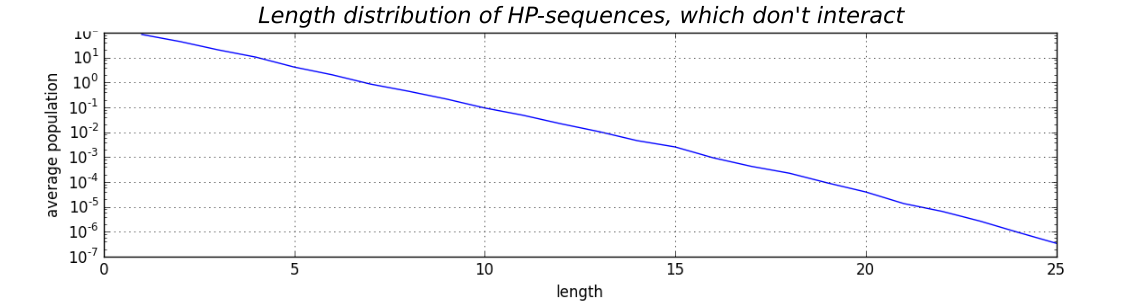
\includegraphics[width=0.9\textwidth]{pictures/flory.png} 
  \caption{We are dealing with an exponential length distribution. 
    Model described in \ref{sec:flory}}
  \label{fig:flory}
\end{figure}

For example let us consider set up, which gives picture above. For this model give the following 
polymer abundance:
\begin{equation}
  \frac{\pq{10mers}}{\pq{1mers}}=10^{-3},\qquad\frac{\pq{20mers}}{\pq{1mers}}=10^{-7}
\end{equation} 
\red{I think here adding maybe another polymerization model and also a couple of variant of 
  ``realistic'' parameters. In some compact way, so that it doesn't take much attention.}

\noindent\red{\textbf{Activity Statement.}} We sought a simple structure based mechanism, which 
would lead to reasonable lengths of polymers information formation, inheritance and complexity of 
the system.

\noindent\red{\textbf{Forecasting Statement.}}Here, we address both the Flory problem of reaching 
long chains, and the informational problem

\gray{\textbf{Old.}\\
We are interested in the conceptual problem of how early prebiotic polymerization processes 
might have led from short nonspecific random sequences to sequences that are longer and more specific.  
We frame a physics question, rather than a chemical one:  we are looking for a simple system, 
which would be able to qualify for ``being alive'',  while staying simple enough to be formed 
spontaneously. In this framework precise chemical composition is not of a great importance, and 
our agents(?) don't have to be chemical similar or related to ones in the prebiotic world.}

\gray{
There is a large body of literature that addresses prebiotical plausibility of various chemical 
systems. \cite{Orgel,}.  
We, on the other hand, are focused here on matters of principle of the possible mechanisms 
by which informational polymers could have arisen from random polymers.  
}

\gray{
Some important modeling works have considered the matter of how homopolymers or random 
polymers could be made long enough for biochemistry to take over \cite{}.  
\blue{These are intended to address the well-known problem that neither DNA \cite{} nor proteins 
  \cite{} nor other potential prebiotic polymers \cite{} are able to break out of what we call the 
  ``Flory problem''. }
By Flory problem, we mean that the main types of polymerizations lead to exponential relationship
between length and abundance \cite{Flory1953,??}.  In particular, a broad range of experiments 
of  polymerizations under pre-biotic conditions show that rarely do DNA molecules or RNA 
or proteins ever reach chain lengths longer than a few monomers long \cite{}. 
 \red{here's an issue that there're experiments, where longer chains were reached by means
   of some prebiotically plausible catalysts: \cite{}. Address this issue.}
And, these are much too short to initiate biology. 
}





 





\section{HP model Foldamers}
Here, we adopt the HP model -- one of the simplest models of proteins for which sequence 
space is well understood.   
\paragraph{HP model setup} 
\begin{itemize}
 \item It is a two dimensional square lattice model of protein folding
 \item It has 2 types of monomers: hydrophobic (H) and polar (P). Hence the name.
 \item \red{A couple of other details, figs, etc.}
\end{itemize}
\red{\dots}  It is 2D, but this simplification is  is known to be largely innocuous 
with respect to predicting protein-like properties, and yet is an important simplification for 
understanding full sequence-spaces and folding.   

\blue{The basic previous finding is that even sequence heteropolymers that are as simple as HP 
will often fold up, even as short chains, because of their ability to form hydrophobic contacts in 
water.  Such short HP chains will not necessarily have unique ``ground states'' \red{(in the 
definitions section. need to be separated properly)}; they will often be fairly amorphous 
`oil-drop’-like balls that are ensembles of conformations.  Some HP sequences will fold more 
uniquely than others.  And, importantly, it has been known for many years \cite{lau1989lattice} 
that a relatively large fraction of sequence space will fold to compact structures or compact 
ensemble structures.}


\section{Foldamer catalysts.}
Our central premise is that the same promiscuous hydrophobic interactions that can cause random 
HP heteropolymers to collapse to compact, sometimes folded, structures, will also cause 
polymer-polymer attractions and binding between molecules.  In some cases, a folded HP-mer can 
provide a hydrophobic ``landing site'' for another HP polymer and/or another H monomer.  Here is 
our mechanism of how a foldamer could catalyze the synthesis of another chain \red{[details ...]}  
Of course, these will not be good catalysts.  But, even the weak localization onto a hydrophobic 
surface is sufficient, at only about 1-2 kT per H-H interaction in water, will be sufficient to 
cause translational localization that can reduce a polymerization barrier by that amount (fig 
\ref{fig:assist-barrier}).
\begin{figure}[h!]
  \centering
  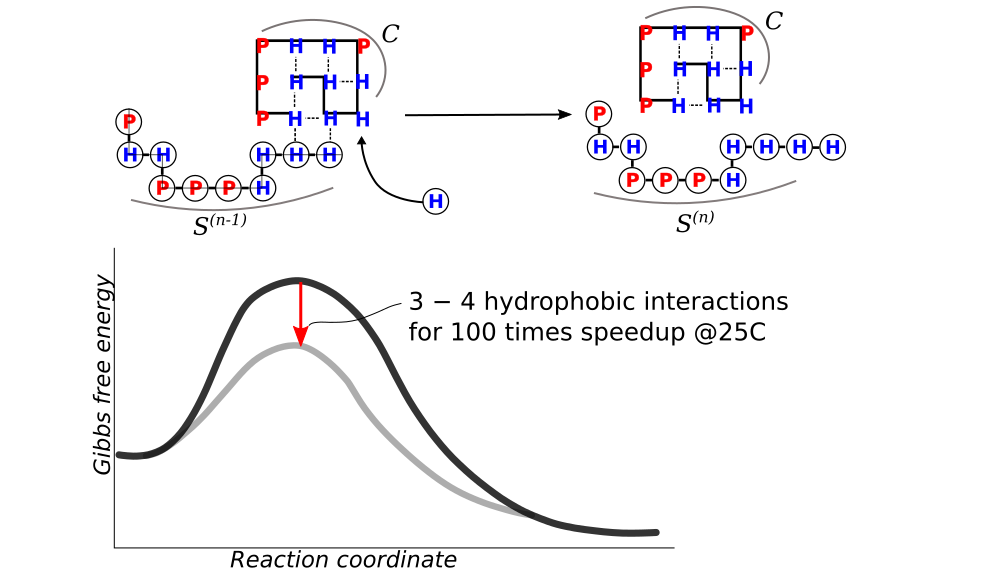
\includegraphics[width=0.75\textwidth]{pictures/assistance-with-barrier.png} 
  \caption{Catalyst $C$ catalyzes a growing of an unfolded hp-polymer. 
           Having just 3-4 hydrophobic contacts is enough to lower an 
           activation barrier for $\propto 100$ times at room 
           temperature.}\label{fig:assist-barrier}
\end{figure}

To see examples HP sequences, which can or cannot be catalysts see fig. \ref{fig:ex-fold-n-cat} 
(a) and (b) correspondingly. The foldamer presented on fig. \ref{fig:ex-fold-n-cat}(a) is also an 
autocatalyst because it has long enough stretch of hydrophobs, which could be formed in a reaction 
of HP-catalysis.
\begin{figure}[h!]
  \centering
  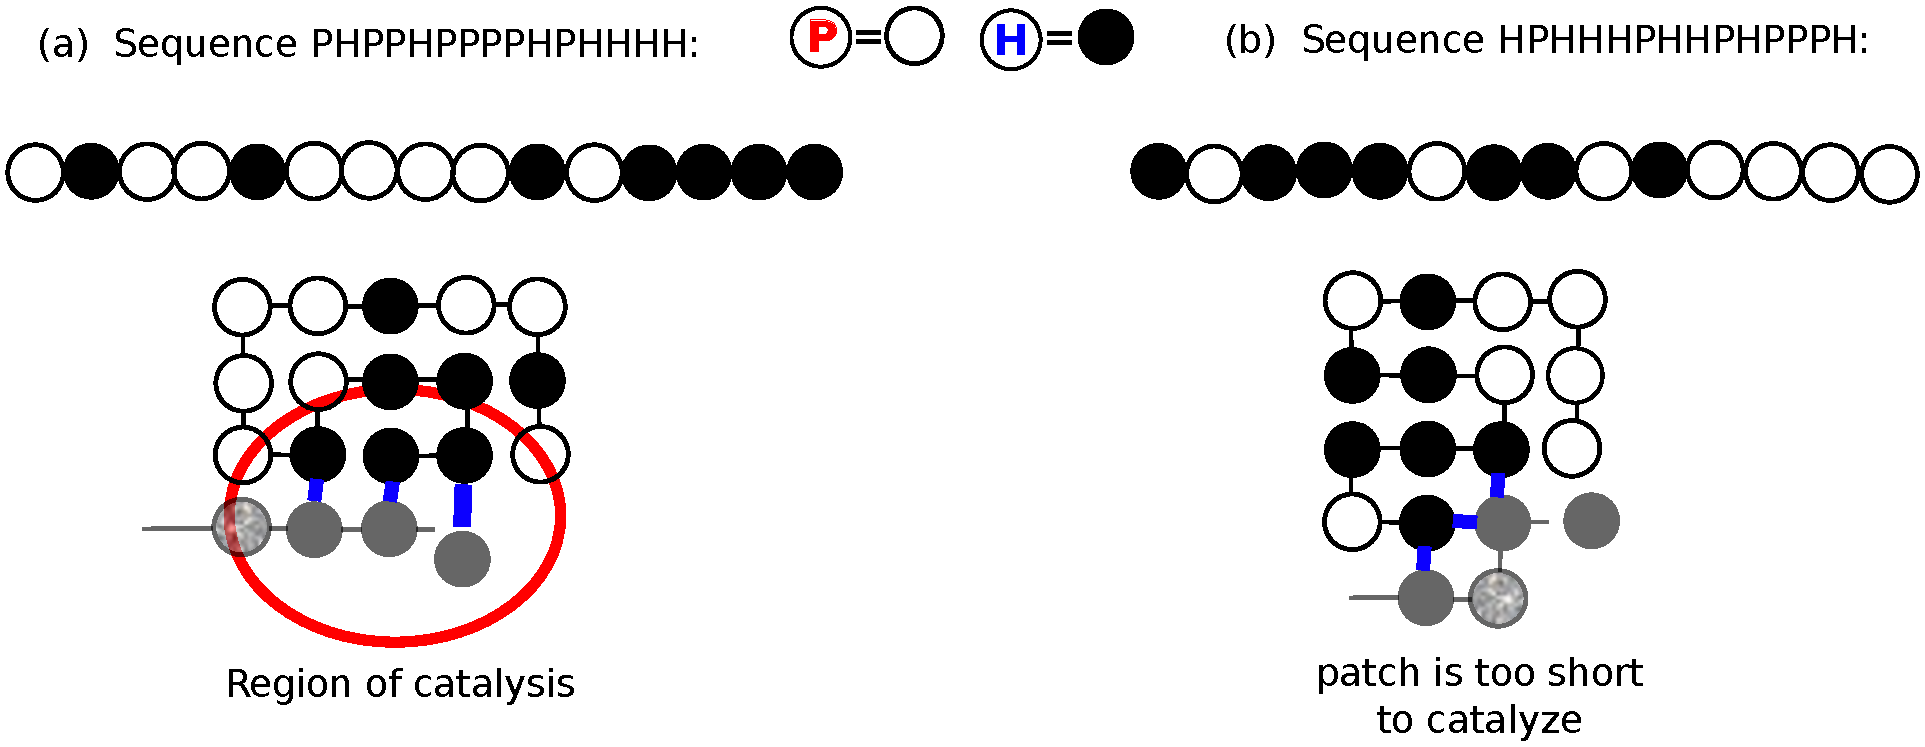
\includegraphics[width=0.95\textwidth]{pictures/example-fold-n-cat.pdf} 
  \caption{...}\label{fig:ex-fold-n-cat}
\end{figure}


\paragraph{Definitions} \red{(split them)}
\begin{itemize}
  \item Folded state is the state which minimizes conformation energy of a chain. 
  It's also has to be a unique state with its energy.
  \item Catalysts are sequences which have a \textit{big enough} hydrophobic patch on its 
  surface. In our 2D case it's a patch of three hydrophobs.
  \item We have a very loose definition of autocatalysts:
  they are the chains which are: capable of catalysis, have at least one of their bonds produced 
  through catalyis.\ref{fig:hp-stat}
\end{itemize}


\section{Proof in the form of simulations}
\red{Some nice figures are being prepared}

\red {\textbf{KD:} Let’s show figures here.  Show how the Flory curve gets shifted.  Show the 
effect of folding alone.  Show how autocats help.  Show how this bridges across from short lengths 
at low concentrations to longer lengths, specific sequences and higher concentrations.}
\section{Maybe some math will go here to support our point of view analytically}


 \newpage
\appendix
\section{Flory problem derivation}\label{sec:flory}
Suppose one has a plenty of monomers either in closed reservoir or in the system that allows 
import of monomers and waste output. Suppose there are also two competing mechanism acting upon 
the system: 
\par (a) Growth: reactions like
\begin{itemize}
  \item (Activated) monomer addition
  \item Ligation of two oligomers
\end{itemize}
\par (b) Degradation: reactions like
\begin{itemize}
  \item Full degradation/leaving a vesicle/dilution
  \item Hydrolysis of bonds of polymers.
\end{itemize}
In systems like these the steady state distribution of length will be exponential
Rate constants: growth=1, import=100, degradation=0.1

 \section{To sort}
 
 \begin{enumerate}
   \item 2D HP lattice model
   \item We look at random sequences
   \item There are a plenty of monomers.   \red{it might be worth reconsidering this one}
   \item ??   \red{consider what other properties are internal for our world}
   \begin{figure}[h!]
     \centering
     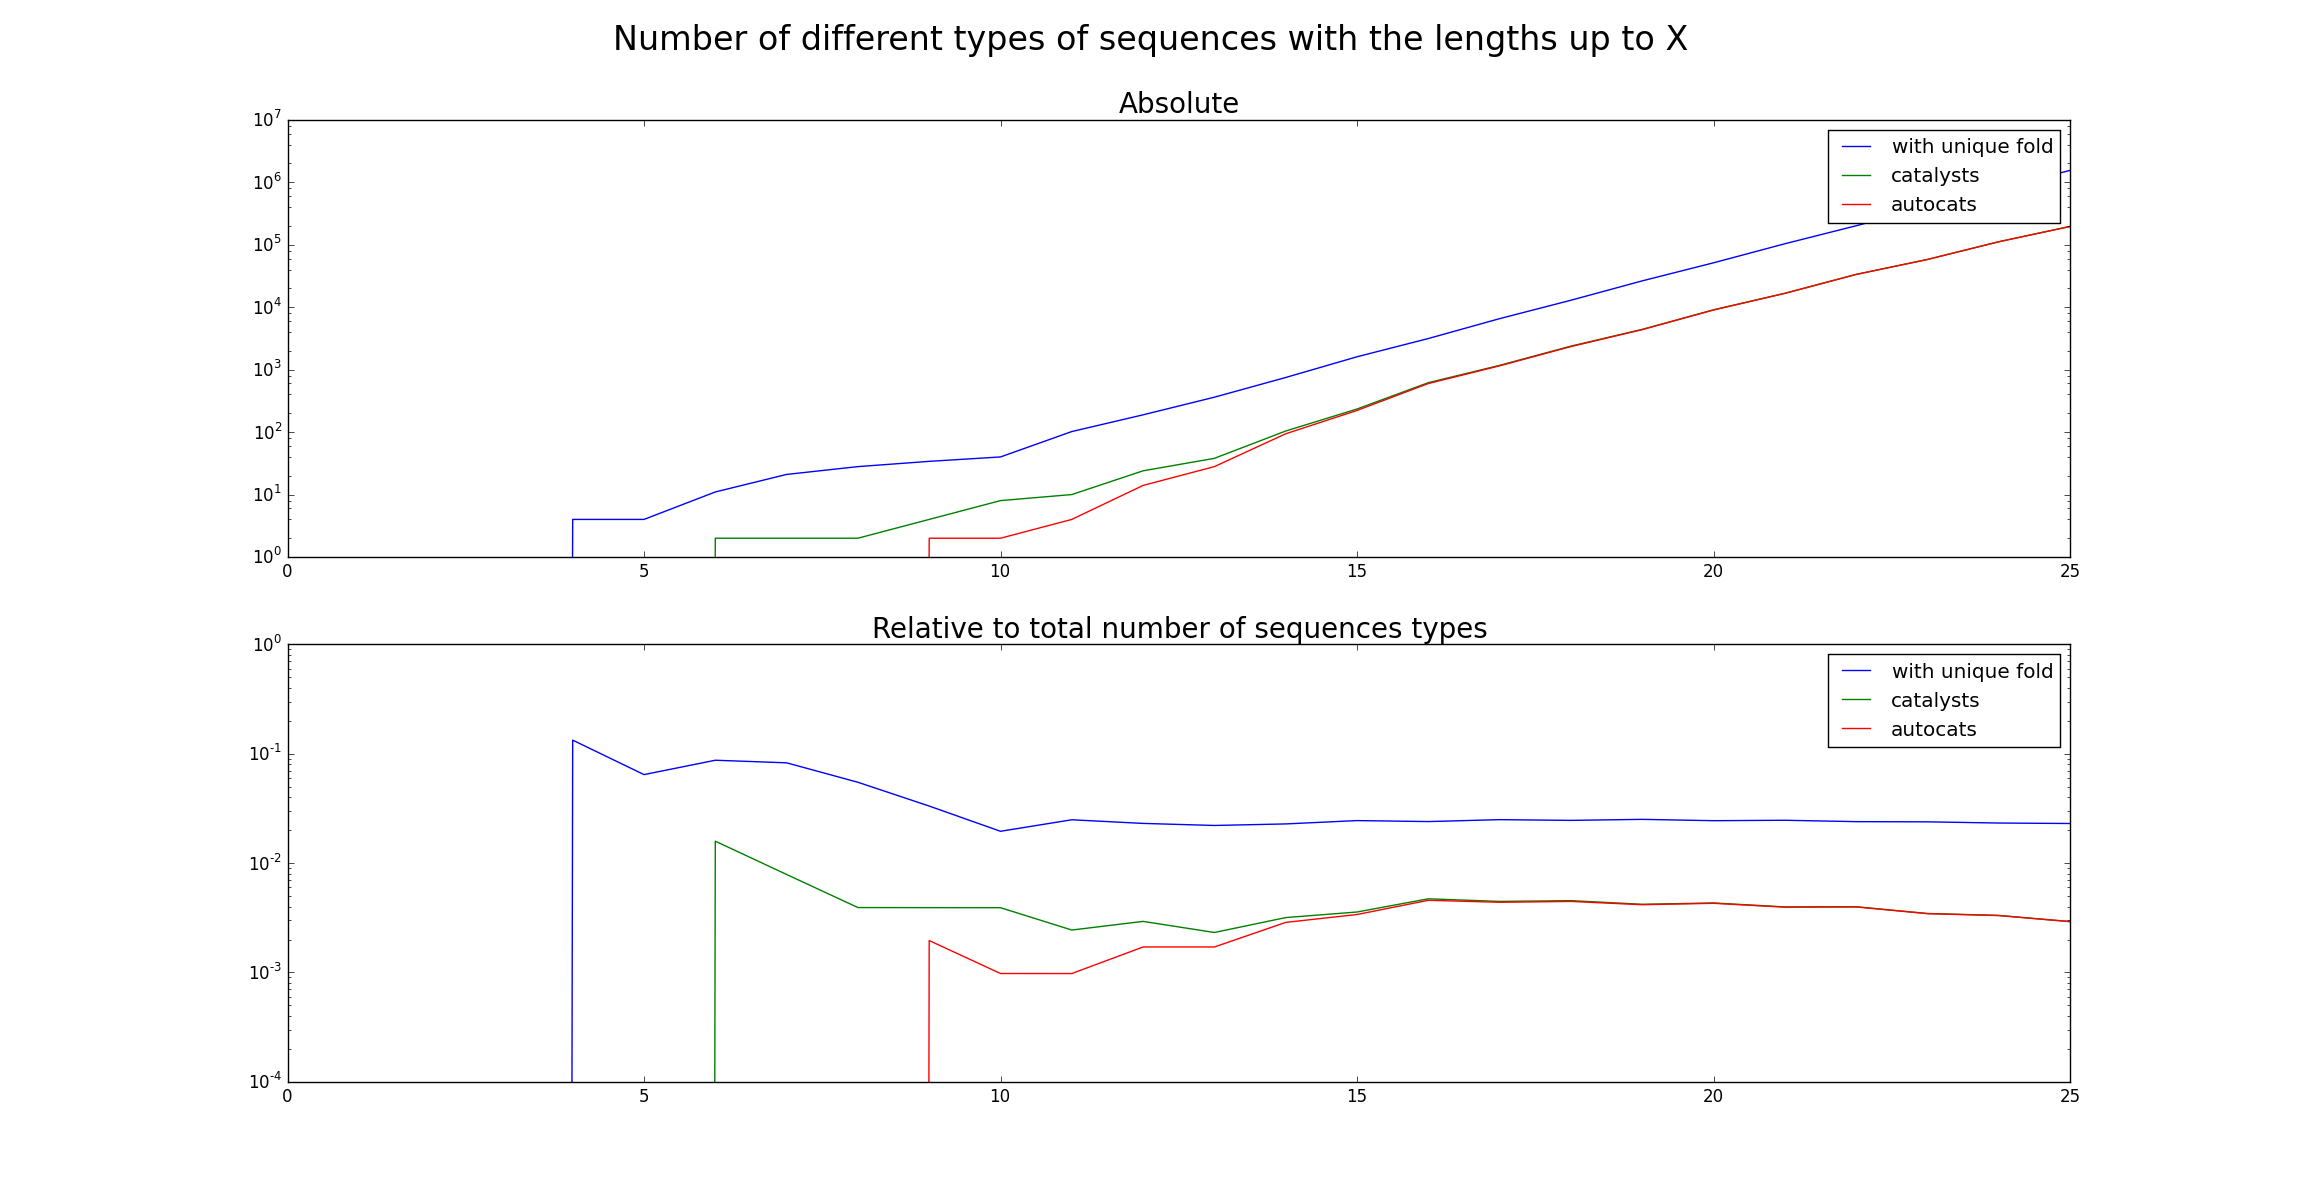
\includegraphics[width=0.9\textwidth]{pictures/hp-statistics.png} 
     \caption{...}\label{fig:hp-stat}
   \end{figure}
   \item This model is sufficient to reach long chains: \red{multiply the graph from 
     fig. \ref{fig:hp-stat} to exponential distribution.}
   \subitem \textbullet Show some dynamics
   \item We don't think of this as whole story. 
   \subitem \textbullet But it shows a mechanism for why seq. heteropolymers can reach some 
   \textit{interesting} state.
 \end{enumerate}

 \bibliography{/data/research/31.mendeleyBibtex/Origins}
 \bibliographystyle{apalike}


\end{document}
